\mode<article>{\usepackage{fullpage}}
\mode<presentation>{\usetheme{Berlin}}
% everyone:
\usepackage[english]{babel}
\usepackage{pgf}
\pgfdeclareimage[height=1cm]{myimage}{filename}

%\usepackage{parskip}
\usepackage{booktabs}
\usepackage[normalem]{ulem}
\useunder{\uline}{\ul}{}
\setlength{\parskip}{\baselineskip} 

% Theme choice:
\usetheme{Madrid}
% Title page details: 
\title[Distal Acupuncture]{Distal Acupuncture: Theory and Practice}
\subtitle{A systems based approach to complex patterns}
\author{Steven Malins, DOM}
\institute{New Mexico Society for Acupuncture and Asian Medicine}
\date{15 September, 2024}
\begin{document}
% Title page frame
\begin{frame}
    \titlepage
\end{frame}

% Outline frame
\begin{frame}[allowframebreaks]{Outline}
    \tableofcontents[hideallsubsections]
\end{frame}



%%%%%% # INTRODUCTION
\section{Introduction}

\begin{frame}{Steven Malins, DOM}
  \begin{figure}
    \centering
    \includegraphics[width=0.9\textwidth]{img/westie01.jpg}
  \end{figure}
\end{frame}

\begin{frame}{Who am I?} %1.1
  \textbf{\Large My Experience}
  \begin{itemize} \itemsep1em
  \item Licensed for 10 years
  \item Community acupuncture for 3 years, 20+ patients per shift
  \item Community acupuncture for indigenous elders 2x month
  \end{itemize}
\end{frame}

\begin{frame}{References}
  \begin{itemize} \itemsep1em
  \item Deadman, P., Al-Khafaji, M., \& Baker, K. (2007). A manual of acupuncture. Journal of Chinese Medicine.
  \item Kuwahara, T. K. (2003). Traditional Japanese Acupuncture: Fundamentals of Meridian therapy. Paradigm Publications.
  \item O'Connor, J., \& Bensky, D. (1981). Acupuncture: A comprehensive text. Editora Roca.
  \item Tan, T. (2007). Acupuncture 1, 2, 3.
  \end{itemize}
\end{frame}

\begin{frame}{Why Distal Acupuncture?} %1.2
  \begin{center}
    \pause
    \begin{enumerate}
    \item \LARGE Distal acupuncture works!
      \pause
    \item \LARGE Patients with mobility issues
      \pause
    \item \LARGE Wide range of conditions treated
      \pause
    \item \LARGE Systems based, treat patterns not symptoms
    \end{enumerate}
  \end{center}
\end{frame}

\begin{frame}{How does acupuncture work?} %1.3
  \textbf{\Large Endorphin Acupuncture Analgesia (AA)}
  \begin{itemize}
  \item AA Works much better than placebo
    \begin{itemize}
    \item 55\% to 85\% of cases
    \item Morphine ~ 75\% of cases!
    \item Placebo ~ 30\% of cases
    \end{itemize}
  \end{itemize}
  \begin{quote}
    In summary, acupuncture stimulates nerve fibers in the muscle, which send impulses to the spinal cord and activates three centers (spinal cord, midbrain, and hypothalamus-pituitary) to cause analgesia.
  \end{quote}

  Stux, G., \& Pomeranz, B. (2012). Basics of acupuncture. Springer Science \& Business Media. 
  
\end{frame}

\begin{frame}{Ling Shu} %1.4
  \begin{quote}
    When there is a perverse disease with pain which goes along both sides of the backbone to reach the top of the head, and the head nods with heaviness, the eyes are blurred, and loins and spine are stiff and rigid, treat the Leg Major Yang at the point in the middle of the crease of the knee.
  \end{quote}

  Jing-Nuan, W. (Trans.). (2011). Ling Shu: Or the spiritual pivot. The Taoist Center.
\end{frame}

\begin{frame}{Diagnosis} %1.5
  \newtheorem{t1.4}{TCM Diagnosis}
  \begin{t1.4}
    TCM diagnosis, eg ``spleen qi vacuity'' works for herbs but is not useful for acupuncture
  \end{t1.4}

  \vspace{1em}

  \begin{quote}
    What is your diagnosis? Spleen Qi Deficiency?!
  \end{quote}

\end{frame}

\begin{frame}{When to use Distal Acupuncture?} %1.6
  \newtheorem{t1.5}{What Can Distal Acupuncture Treat?}
  \begin{t1.5}
    Distal Acupuncture can treat (almost) any pattern/condition!
  \end{t1.5}

  \begin{itemize}
  \item Distal Acupuncture affects cells in Mid-Brain and Pituitary Hypothalamus
  \item All 5 shu points are distal on all 12 meridians
  \item Treating patterns and not symptoms reduces number of needles and increases effectiveness!
  \end{itemize}

\end{frame}

\begin{frame}{When NOT to use Distal Acupuncture} %1.7
  
  \textbf{\Large When to avoid Distal Acupuncture}
  \begin{itemize} \itemsep1.5em
  \item Open wounds near points needed
  \item Chronic pain not responsive to DA
  \item Medical Emergencies!
  \end{itemize}

  \newtheorem{t1.6}{Case Study}
  \begin{t1.6}
    MC: abdominal pain, progressively worse past 24h; rebound tenderness; temperature 100.0
  \end{t1.6}
  
\end{frame}

\begin{frame}{Case Study 0.1} %1.8a
  \textbf{\Large 65F MC: Neck pain}
  
  \textbf{\large Subjective}
  
  \textbf{HPI:} Neck pain started ``a few days ago'' worse with neck flexion; patient describes pain as ``stiff''; radiates to whole head; severity 6 out of 10

  \textbf{\large Objective}
  
  \textbf{P:} vacuous; deep; rapid

  \textbf{PE:} BP 110/76, PR 87, T 99.7; patient is slow to answer questions; otherwise unremarkable

\end{frame}

\begin{frame}{Case Study 0.1} %1.8b
  \newtheorem{dx}{Diagnosis}
  \newtheorem{pln}{Plan}
  \textbf{\Large 65F MC: Neck pain}

  \begin{dx}
    \textbf{Suspected Meningitis!}
  \end{dx}

  \begin{pln}
    Refer to ER for lumbar puncture to confirm or rule out Meningitis
  \end{pln}

\end{frame}
  
\begin{frame}{Discussion}
  \begin{figure}
    \centering
    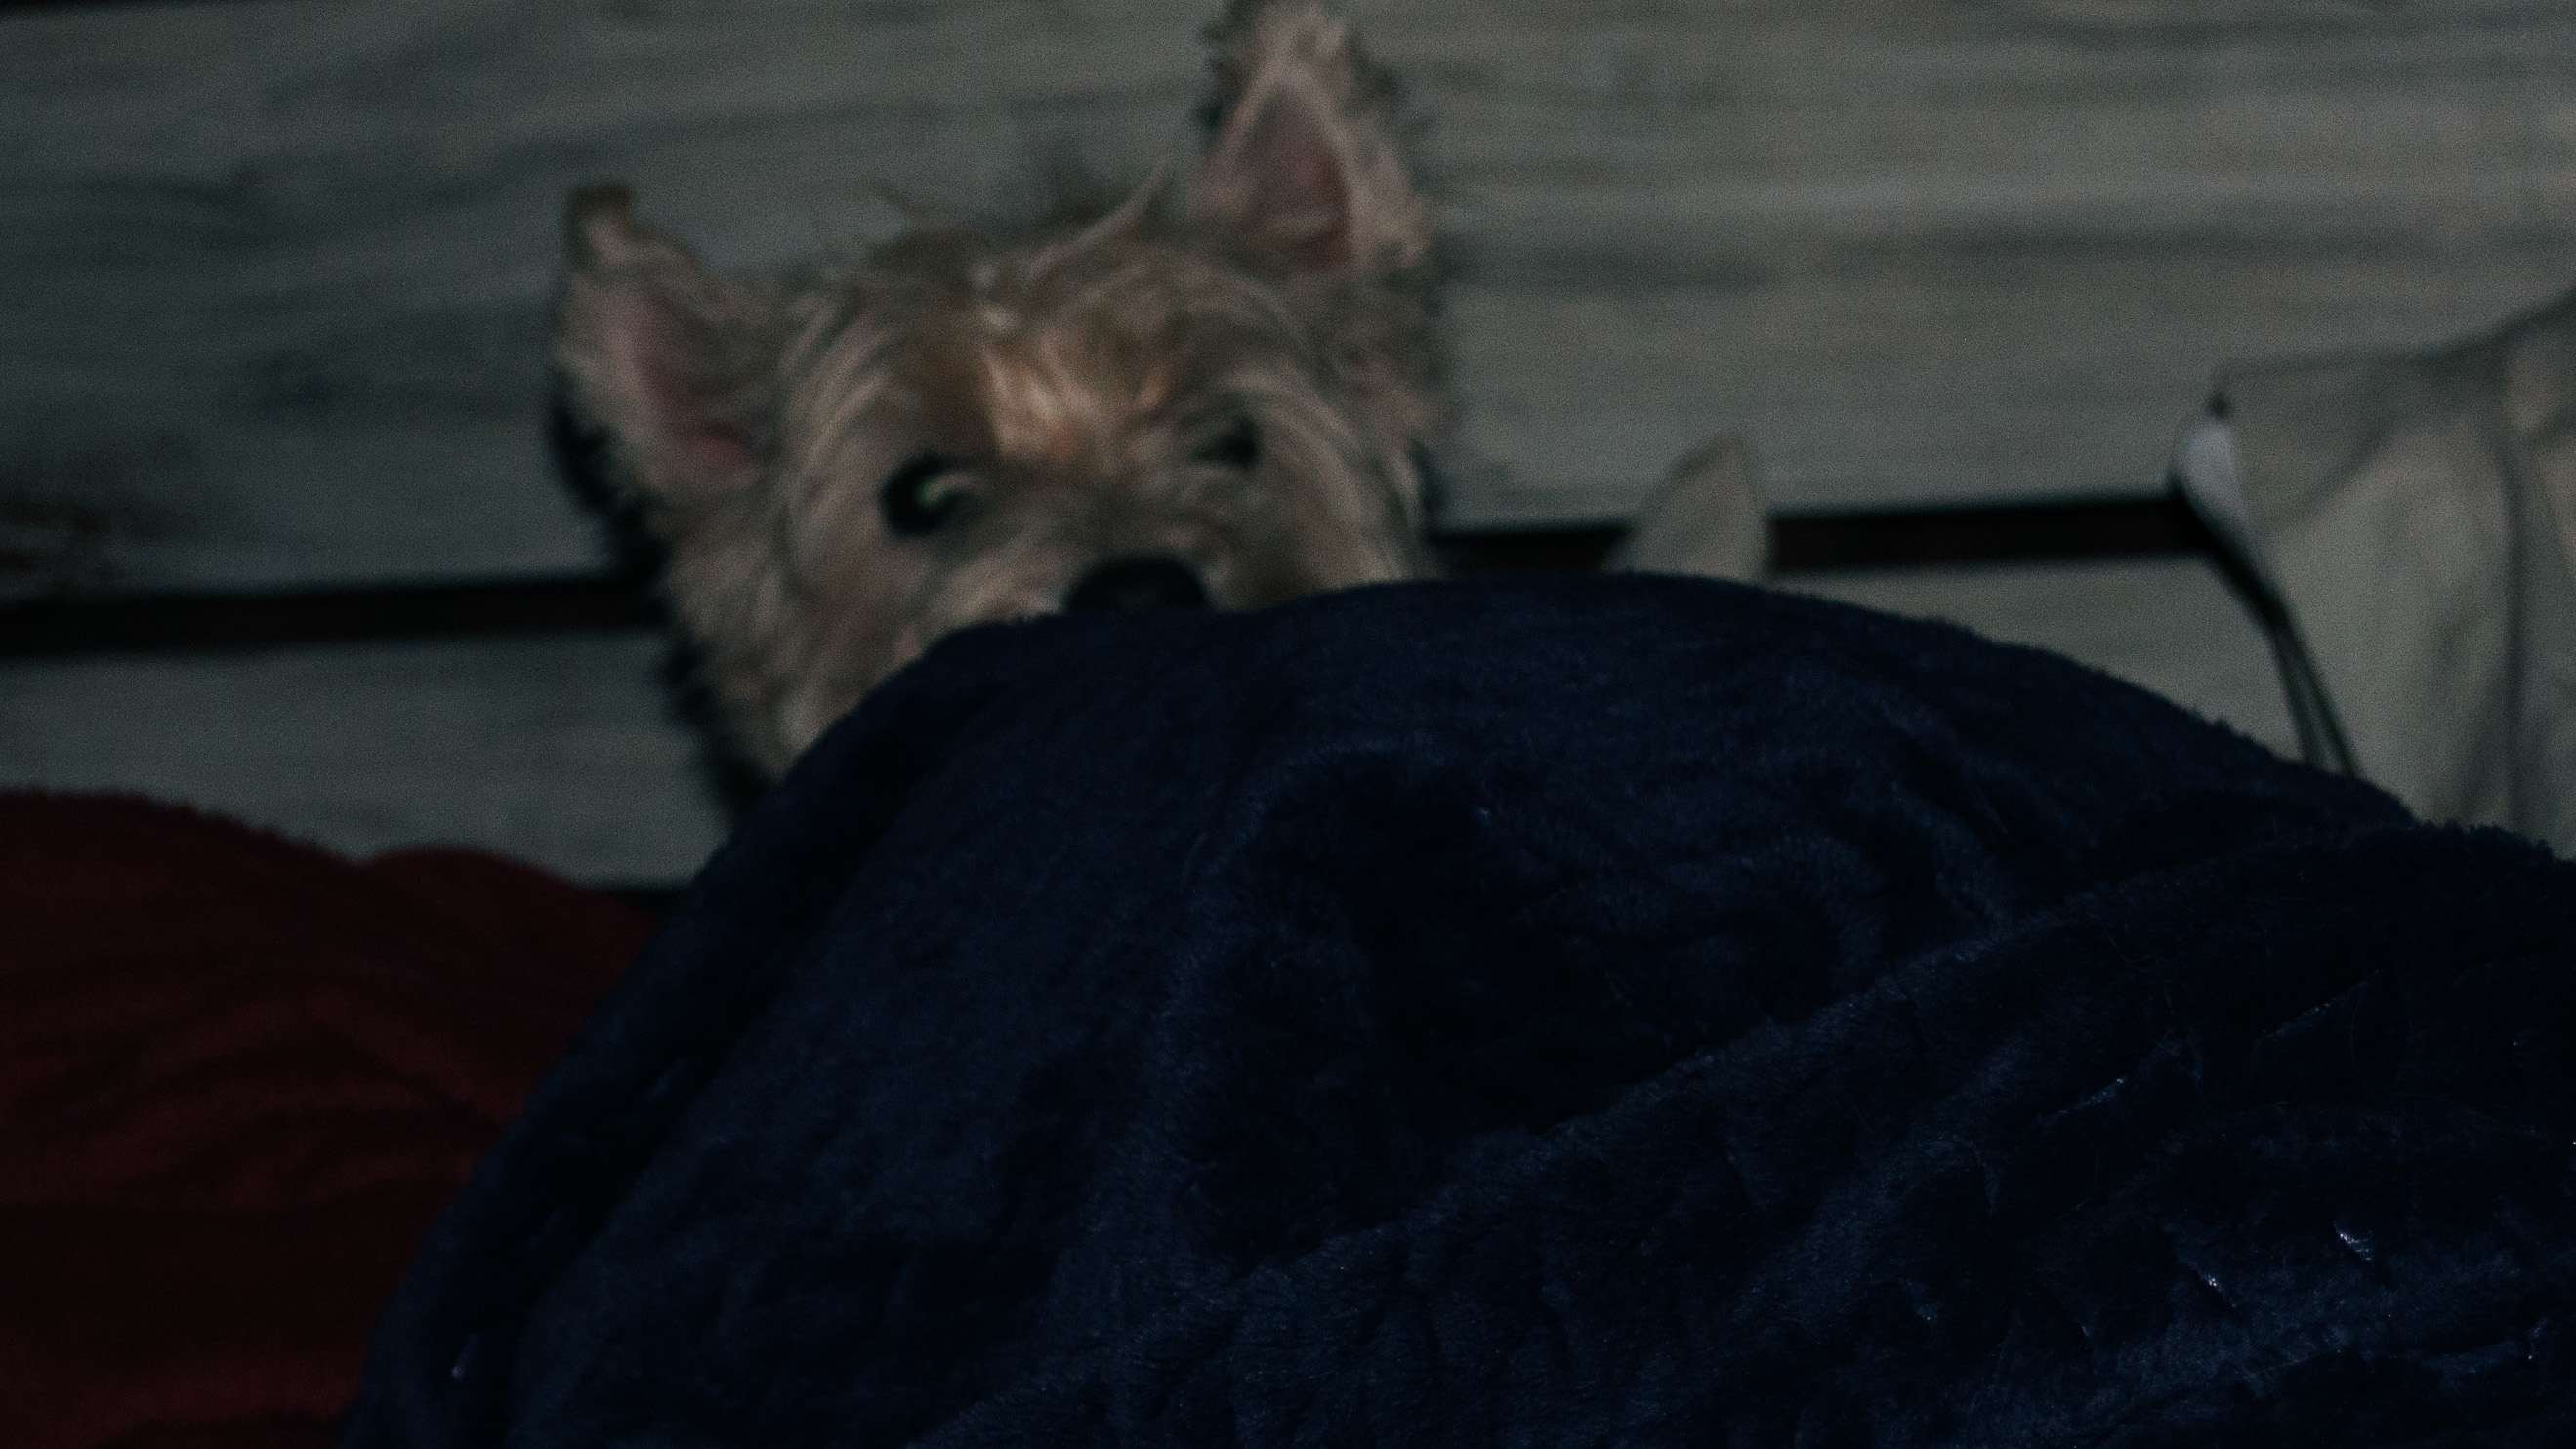
\includegraphics[width=0.9\textwidth]{img/westie02.jpg}
  \end{figure}
\end{frame}

%%%%%% # Miriam Lee
\section{Miriam Lee 10 Points}          

\begin{frame}{Ten Needle Technique}
\begin{quote}     
When the stomach and spleen, the centraJ jiao, are attacked by
emotion, pure qi cannot ascend to the brain, and theevil qi, the
waste, cannot descend. It will remain stuck in the stomach.
\end{quote}

Lee, M. (1992). Insights of a senior acupuncturist. Blue Poppy
Enterprises.

\end{frame}

\begin{frame}{Miriam Lee Magic 10}
\begin{itemize}
\item ML treated up to 17 patients per hour!
\item Many clinical applications
\item ``never fails'' says Miriam Lee
\end{itemize}

\begin{table}[]
\begin{tabular}{@{}lll@{}}
\toprule
LI-11 & Pool at the Crook (Qu Chi)            & Disperse             \\
LI-4  & Joining Valley (He Gu)                & Disperse             \\
LU-7  & Broken Sequence (Lie Que)             & Disperse             \\
ST-36 & Leg Three Miles (Zu San Li)           & Tonify (Or Disperse) \\
SP-6  & Three Yin Intersection (San Yin Jiao) & Tonify               \\ \bottomrule
\end{tabular}
\end{table}

\end{frame}

\begin{frame}{Broken Sequence}

\large{Lung 7 :: Broken Sequence}

\begin{itemize}
\item Luo Connecting point of Lung Hand Greater Yin
\item Confluent Point of the Conception Vessel
\item Gao Wu Command Point (head and neck)
\item Ma Dan -Yang Heavenly Star Point
\end{itemize}

\vspace{1em}

\begin{quote}
If we think of the alternative name Broken Sequence we can see how this point is good for breaking patterns of grief and loss.
\end{quote}

\end{frame}

\begin{frame}{Pool at the Crook}

\large{Large Intestine 11 :: Pool at the Crook}

\begin{itemize}
\item Earth of Metal and Uniting Point of Large Intestine
\item Sun Si-Miao Ghost Point
\item Ma Dan-Yang Heavenly Star Point
\end{itemize}

\vspace{1em}

Clears heat, cools the blood, eliminates wind, drains damp, relieves itching

\end{frame}

\begin{frame}{Joining Valley}

\large{Large Intestine 4 :: Joining Valley}

\begin{itemize}
\item Source point of the Large Intestine Hand Greater Yin
\item Gao-Wu Command Point (face)
\item Ma Dan-Yang Heavenly Star Point
\end{itemize}

\vspace{1em}

Points on the thumb and big toe (eg LI-4 and LR-3) show greater response in the subcortex than other points on fingers and toes. Reflexology also recognizes these areas as having an effect on the head and master regletory endocrine glands in the head. 

\end{frame}


\begin{frame}{Leg Three Miles}

\large{Stomach 36 :: Leg Three Miles}

\begin{itemize}
\item Earth of Earth and uniting point of Stomach Foot Yang Brightness
\item Gao-Wu Command Point (abdomen)
\item Ma Dan-Yang Heavenly Star Point
\item Point of the Sea of Water and Grain
\end{itemize}

\vspace{1em}

Earth of Earth Leg Three Miles tonifies and adjusts the qi and blood of the entire body!

\end{frame}

\begin{frame}{Three Yin Intersection}

\large{Spleen 6 :: Three Yin Intersection}

\begin{itemize}

\item \textbf{Spleen}
\begin{itemize}
\item Drains Damp; improves T \& T
\item Reverses sinking Qi (eg uterine prolapse)
\item Improves Spleen's ability to hold blood
\end{itemize}

\item \textbf{Kidney}
\begin{itemize}
\item Harmonizes Lower Burner
\item Regulates urination
\end{itemize}

\item \textbf{Liver}
\begin{itemize}
\item Soften and harmonize Liver
\item Nourish Liver blood
\end{itemize}

\item Tonify all five Zang by tonifying Spleen
\end{itemize}

\end{frame}

\begin{frame}{ML Magic 10}

\begin{itemize}

\item \textbf{Primary Treatment}
\begin{itemize}
\item Allergies
\item Auto-immune disorders
\item Depression
\end{itemize}

\item \textbf{Can Also Treat}
\begin{itemize}
\item Hypertension
\item Asthma
\item Pneumonia (ML says tx Q4H)
\end{itemize}

\item \textbf{Too many main complaints} eg: ``everything hurts!''

\end{itemize}

\end{frame}

\begin{frame}{Case Study 1}
  \textbf{\Large 67F MC: Back pain; and knee pain; and migraines...}
  
  \textbf{\large Subjective}
  
  \textbf{HPI:} Patient states ``everything hurts, I can barely get out of bed'' progressively worse for many years but much worse the past six months; ``nothing seems to help''; ``like dragging my self through molasses''; whole body pain; severity 8 out of 10 today up to 10 out of 10

  \textbf{\large Objective}
  
  \textbf{P:} vacuous; deep; rapid; minute pulse weak in all positions

  \textbf{PE:} A\&O x4, vitals unremarkable, no focal neurological deficits, skin slightly cool and dry

\end{frame}

%%%%%% # Acupuncture 1,2,3
\section{Acupuncture 1,2,3}

\begin{frame}{Acupuncture 1,2,3}
  \begin{itemize}
  \item Dr Richard Tan
  \item Three Steps:
    \begin{itemize} \itemsep1em
    \item \textbf{Step 1:} Diagnose the Sick Meridian
      \begin{itemize}
      \item Inspection
      \item Auscultation
      \item Inquiry
      \end{itemize}
    \item \textbf{Step 2:} Determine Treating Meridians
      \begin{itemize}
      \item{5 Systems}
      \end{itemize}
    \item \textbf{Step 3:} Point selection
    \end{itemize}
  \end{itemize}

  \begin{quote}
    An affected meridian may indicate soley a physical pain, or may be an indication of an internal issue
  \end{quote}
\end{frame}

\begin{frame}{System I}
  \newtheorem{ns}{Needle Side}
  \textbf{\Large Meridian Name-Sharing}

  \begin{table}[]
    \begin{tabular}{@{}ll@{}}
      \toprule
      Meridian 1                    & Meridian 2                \\ \midrule
      Lung Hand TaiYin              & Spleen Foot TaiYin        \\
      Large Intestine Hand YangMing & Stomach Foot YangMing     \\
      Heart Hand ShaoYin            & Kidney Foot ShaoYin       \\
      Small Intestine Hand TaiYang  & Bladder Foot TaiYang      \\
      Triple Burner Hand ShaoYang   & Gallbladder Foot ShaoYang \\
      Pericardium Hand JueYin       & Liver Foot JueYin         \\ \bottomrule
    \end{tabular}
  \end{table}
  \begin{ns}
    Opposite Side
  \end{ns}
\end{frame}

\begin{frame}{System II}
  \textbf{\Large Branching Meridians}
  \begin{table}[]
    \begin{tabular}{@{}ll@{}}
      \toprule
      Meridian 1                    & Meridian 2                 \\ \midrule
      Lung Hand TaiYin              & Bladder Foot TaiYang       \\
      Large Intestine Hand YangMing & Liver Foot JueYin          \\
      Heart Hand ShaoYin            & Gallbladder  Foot ShaoYang \\
      Small Intestine Hand TaiYang  & Spleen Foot TaiYin         \\
      Triple Burner Hand ShaoYang   & Kidney Foot ShaoYin        \\
      Pericardium Hand JueYin       & Stomach Foot YangMing      \\ \bottomrule
    \end{tabular}
  \end{table}

  \begin{ns}
    Either Side
  \end{ns}
\end{frame}

\begin{frame}{System III}
  \textbf{\Large Interior Exterior}
  \begin{table}[]
    \begin{tabular}{@{}ll@{}}
      \toprule
      Meridian 1  & Meridian 2      \\ \midrule
      Lung        & Large Intestine \\
      Heart       & Small Intestine \\
      Pericardium & Triple Burner   \\
      Spleen      & Stomach         \\
      Kidney      & Bladder         \\
      Liver       & Gallbladder     \\ \bottomrule
    \end{tabular}
  \end{table}

  \begin{ns}
    Opposite Side
  \end{ns}
\end{frame}

\begin{frame}{System IV}
  \textbf{\Large Clock Opposites}

  \begin{figure}
    \centering
    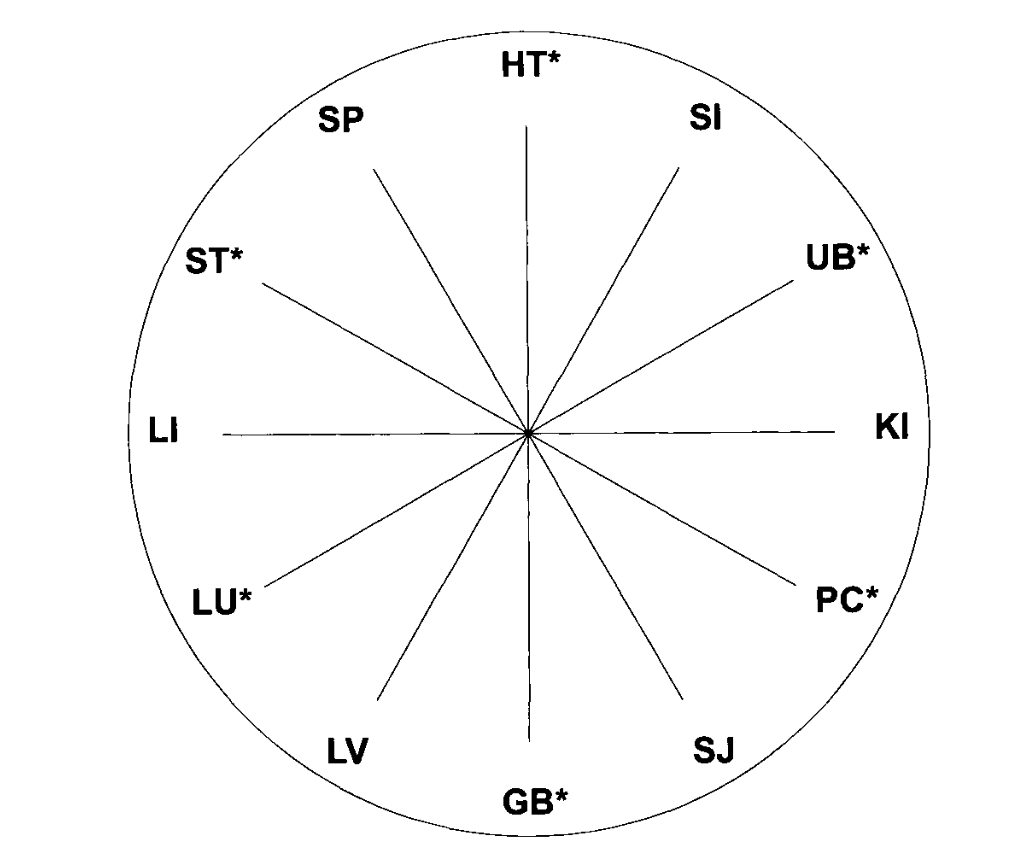
\includegraphics[height=0.5\textheight]{img/mclock.png}
  \end{figure}

  \begin{ns}
    Either Side
  \end{ns}
\end{frame}

\begin{frame}{System V}
  \textbf{\Large Clock Neighbors}

  \begin{table}[]
    \begin{tabular}{@{}ll@{}}
      \toprule
      Meridian 1                        & Meridian 2                    \\ \midrule
      Lung                              & Liver                         \\
      \textit{\textbf{Large Intestine}} & \textit{\textbf{Stomach}}     \\
      Spleen                            & Heart                         \\
      \textit{\textbf{Small Intestine}} & \textit{\textbf{Bladder}}     \\
      Kidney                            & Pericardium                   \\
      \textit{\textbf{Triple Burner}}   & \textit{\textbf{Gallbladder}} \\ \bottomrule
    \end{tabular}
  \end{table}
  
  \begin{ns}
    Opposite Side
  \end{ns}
\end{frame}

\begin{frame}{Imaging I}
  \begin{table}[]
    \begin{tabular}{l|ll}
      {\ul \textbf{Needled Area}} & \multicolumn{2}{c}{{\ul \textbf{Sick Area}}}                                    \\ \hline
      & \multicolumn{1}{c}{\textit{Image}} & \multicolumn{1}{c}{\textit{Reverse Image}} \\
      Finger                      & Genitals anus                      & Top of head                                \\
      Hand                        & Coccyx, sacrum                     & Base of head                               \\
      Wrist                       & Bladder L-S                        & Neck                                       \\
      Forearm                     & Low AB and Back                    & Upper ab and back                          \\
      Elbow                       & Umbilicus, L-2, waist              & Umbilicus, L-2, waist                      \\
      Upper arm                   & Upper ab and back                  & Low AB and Back                            \\
      Shoulder                    & Base of head                       & Coccyx, sacrum                             \\
      Top of shoulder             & Top of head                        & Genitals anus                             
    \end{tabular}
  \end{table}
\end{frame}

\begin{frame}{Imaging II}
  \begin{table}[]
    \begin{tabular}{l|ll}
      {\ul \textbf{Needled Area}} & \multicolumn{2}{c}{{\ul \textbf{Sick Area}}}                                    \\ \hline
      & \multicolumn{1}{c}{\textit{Image}} & \multicolumn{1}{c}{\textit{Reverse Image}} \\
      Toe                         & Genitals anus                      & Top of head                                \\
      Foot                        & Coccyx, sacrum                     & Base of head                               \\
      Ankle                       & Bladder L-S                        & Neck                                       \\
      Lower Leg                   & Low AB and Back                    & Upper ab and back                          \\
      Knee                        & Umbilicus, L-2, waist              & Umbilicus, L-2, waist                      \\
      Upper Leg                   & Upper ab and back                  & Low AB and Back                            \\
      Hip                         & Base of head                       & Coccyx, sacrum                             \\
      Top of Hip                  & Top of head                        & Genitals anus                             
    \end{tabular}
  \end{table}
\end{frame}

\begin{frame}{Acupuncture 1,2,3 Example}
  \newtheorem{s1}{Diagnose the Sick Meridian}
  \newtheorem{s2}{Determine Treating Meridian}
  \newtheorem{s3}{Point Selection}
  \LARGE{Back Pain}

  Area of Discomfort: Paraspinal pain from L3 to L4, left side
\end{frame}
\begin{frame}{1,2,3}
  \begin{s1}
    Bladder meridian, left side
  \end{s1}

  \begin{s2}
    System 1 \& 5: Small Intestine\\
    System 2 \& 4: Lung\\
    System 3: Kidney
  \end{s2}

  \begin{s3}
    SI 7 to SI 8 right side \\
    LU 5 to LU 6 either side \\
    KI 8 to KI 10 right side \\
  \end{s3}
\end{frame}

\begin{frame}{Acupuncture 1,2,3 Example}
  \textbf{\LARGE{Bells's Palsy}}

  Area of Discomfort: Facial paralysis and pain, with difficulty moving the eye, cheek, and mouth, right side.
\end{frame}

\begin{frame}{Step 1 and 2}
  \begin{s1}
    Gallbladder, Stomach, Large Intestine, Triple Burner, right side
  \end{s1}

  Step 2: Determine Treating Meridians

  \begin{table}[]
    \begin{tabular}{@{}lllll@{}}
      \toprule
      & GB                & ST                & LI                & TB                \\ \midrule
      \textbf{I}   & TB                & LI                & ST                & GB                \\
      \textbf{II}  & HT                & {\ul \textbf{PC}} & {\ul \textbf{LR}} & KD                \\
      \textbf{III} & {\ul \textbf{LR}} & SP                & LU                & {\ul \textbf{PC}} \\
      \textbf{IV}  & HT                & {\ul \textbf{PC}} & KD                & SP                \\
      \textbf{V}   & TB                & LI                & ST                & GB                \\ \bottomrule
    \end{tabular}
  \end{table}
\end{frame}

\begin{frame}{Whole Back Pain}
  \Large Dr Tan balance method for whole back, from his book \textit{Acupuncture, 1,2,3}

  \begin{table}[]
    \begin{tabular}{@{}ll@{}}
      \toprule
      Left                   & Right                      \\ \midrule
      LU-5, PC-3, HT-3, HT-7 & Ling Gu, Da Bai, Zhong Bai \\
      GB-41, UB-65           & KI-3, KI-10, SP-6, LR-5    \\ \bottomrule
    \end{tabular}
  \end{table}

\end{frame}
%%%%%% # Global Balance
\section{Global Balance}

\begin{frame}{5 Transport Points}

\begin{quote}
The bloood pulses are widely distributed at the shu points. They are clear to see and strong to touch
\end{quote}

\begin{table}[]
\begin{tabular}{@{}llllll@{}}
    & Well & Brook & Stream & River & Uniting \\
    & Wood & Fire  & Earth  & Metal & Water   \\
LU  & 11   & 10    & 9      & 8     & 5       \\
SP  & 1    & 2     & 3      & 5     & 9       \\
HE  & 9    & 8     & 7      & 4     & 3       \\
KID & 1    & 2     & 3      & 7     & 10      \\
PC  & 9    & 8     & 7      & 5     & 3       \\
LR  & 1    & 2     & 3      & 4     & 8      
\end{tabular}
\end{table}

\end{frame}

\begin{frame}{5 Transport Points}

\begin{quote}
The six bowels have six shu points each. Six times six is thirty six. 
\end{quote}

\begin{table}[]
\begin{tabular}{@{}llllll@{}}
   & Well  & Brook & Stream & River & Uniting \\
   & Metal & Water & Wood   & Fire  & Earth   \\
LI & 1     & 2     & 3      & 5     & 11      \\
ST & 45    & 44    & 43     & 41    & 36      \\
SI & 1     & 2     & 3      & 5     & 8       \\
UB & 67    & 66    & 65     & 60    & 40      \\
TB & 1     & 2     & 3      & 6     & 10      \\
GB & 44    & 43    & 41     & 38    & 34     
\end{tabular}
\end{table}

\end{frame}

\begin{frame}{Well Points}
\newtheorem{well}{Well Points}
\begin{well}
When the disease is at the viscera, needle the well point
\end{well}

\begin{itemize}
\item Fullness below the heart
\item Diseases of the viscera
\item Channel disorders
\end{itemize}

\vspace{0.5em}

Also used to restore conciousness.

\end{frame}

\begin{frame}{Brook Points}
\newtheorem{brook}{Brook Points}
\begin{brook}
If the disease manifests as a change in coulor, needle the brook point
\end{brook}

\begin{itemize}
\item Heat in the body
\item Changes in complexion
\item Diseases of the Yang channels
\end{itemize}

\vspace{0.5em}

SI-2 strongly clears heat from the head, mumps, tinnitus, swelling of the cheek, pain of the neck, nosebleed.

\end{frame}

\begin{frame}{Stream Points}
\newtheorem{stream}{Stream Points}
\begin{stream}
When disease attacks intermittently, needle the stream point
\end{stream}

\begin{itemize}
\item Diseases manifesting intermittently
\item heaviness of the body and pain in the joints
\item disorders of the viscera (with Brook points)
\end{itemize}

\vspace{0.5em}

Yin channels \textbf{Stream} points are also \textit{Source} points. Becuase of this \textit{they are the most important point on their respective channels.}

\end{frame}

\begin{frame}{River Points}
\newtheorem{river}{River Points}
\begin{river}
When the disease manifests as changes in the patient's voice, needle the river point
\end{river}

\begin{itemize}
\item Dyspnoea, cough, chills, and fever
\item Diseases manifesting in the patient's voice
\item Diseases of the sinews and bones (yin channels) 
\end{itemize}

\vspace{0.5em}

HE-4, PC-5, SJ-6 for sudden loss of speech. GB-38 lumbar pain ``like a small weight in the middle of the back'' 

\end{frame}

\begin{frame}{Uniting Points}
\newtheorem{unite}{Uniting Points}
\begin{unite}
If there is disease of the stomach and irregular appetite, needle the uniting point
\end{unite}

\begin{itemize}
\item Rebellious qi and diarrhoea
\item Diseases of the bowels
\item Diseases of the king (yang channels) 
\end{itemize}

\vspace{0.5em}

SP-9 for sudden turmoil disorder due to dampness; UB-39 (lower uniting point of the bladder) for retention of urine or difficult urination. 
\end{frame}

%%%%%% ## TaiYin / YangMing
\subsection{Greater Yin :: Yang Brightness}

%%%%%%## ShaoYin / TaiYang
\subsection{Lesser Yin :: Greater Yang}

%%%%%% ## ShaoYang / JueYin
\subsection{Lesser Yang :: Returning Yin}

%%%%%% # Case Studies 1
\section{Case Studies I}

%%%%%% # Five Element Strategies
\section{Five Element Strategies}

%%%%%% ## Toyo Hari
\subsection{Toyo Hari Style}

%%%%%% ## Five Element Style
\subsection{Five Element Style}

%%%%%% ## Four Needle Technique
\subsection{Four Needle Technique}

%%%%%% # Other
\section{Mircosystems}

\subsection{Ear Acupuncture}

\subsection{Scalp Acupuncture}

\subsection{Master Tung: top points}

%%%%%% # Case Studies 2
\section{Case Studies II}

%%%%%% # Questions
\section{Questions?} 

\begin{frame}
% to enforce entries in the table of contents
\end{frame}

\end{document}
